\section{Discussion}
\subsection{Performance of ZIVA}
Dimensionality reduction is an essential step for downstream analysis, such as clustering and trajectory inference. In this study, we proposed a new model for reducing single-cell sequencing data's dimensionality: zero-inflated variational autoencoder (ZIVA) based on the model in VASC. We tested the performance of ZIVA on several datasets and compared it with six other methods. The result shows that ZIVA can achieve better results in some cases, especially for lineage data. 

Some popular methods, such as tSNE, focus on the local structure but cannot preserve the global structure well. It can significantly separate the clusters of the cells but may fail when data are continuously distributed. Some methods try to keep global structure by maximize the explainable variations but fail to preserve subtle local structures such as PCA. ZIVA has a good balance between local structure and global structure. The result shows that ZIVA can recover the subtle batch effects and can also well recover the developmental cell lineages.

Compared with tSNE and UMAP, it is easier to add a new data point to the ZIVA visualization because it does not need to re-run the algorithm with the whole dataset. A shortcoming of ZIVA is the relatively long running time. For the large datasets that contain thousands of cells, ZIVA may cost several hours on a desktop-level computer. It would be better if we can compress the model to reduce the time cost. Also, for the large datasets, some pre-transformation like feature selection of the input matrix is necessary. For example, Seurat select features by highly variable genes \cite{Satija2015}. M3drop \cite{andrews2019m3drop} performs feature selection based on the dropout rate and removes the genes that only affected by technical noises.

Our model is developed based on Variational autoencoder (VAE) and VASC. Compared with VASC, we made more improvements in VAE and got higher performance on most datasets. Firstly, our model is deeper (4 layers) than the VASC (3 layers). Much research has shown that the deeper network has a higher ability to represent complex non-linear functions. We added an optional dropout model (MM model) for modeling the probability of dropout events in scRNA-seq data. The model parameter in VASC is fixed to 1. However, the dropout distribution may vary in different datasets. So, we added the process of parameter fitting in our model. Also, we used mean square error (MSE) as the loss function. Compared with the cross-entropy loss in VASC, MSE is more suitable in regression problems. 

However, some attempts fail. For example, we tried to add a nuclear norm to the matrix output from the decoder but did not get a good result. I have analyzed the reason for the analysis part. We also tried to add the nuclear norm to the latent variables but also failed. Moreover, we tried to use a neuron network to model the dropout function better. However, to realize that, we need to give the matrix from the decoder a powerful constraint to ensure that matrix is close to the actual expression matrix. Nevertheless, we did not find a proper constraint, and the network fails to learn the actual expression matrix. We also tried to build the dynamics of the gene expression, such as in RNA velocity \cite{la2018rna}. If we can define the dynamics of single-cell expression development, we can use the Koopman theory \cite{morton2018deep} and the deep autoencoder structure to recover the dynamics in two dimensionality \cite{lusch2018deep} and thus reduce the dimensionality of the data and show the dynamics of the data points at the same time. However, we failed to find universal dynamics in the single-cell expression data.  

The variational autoencoder is an excellent framework with many possibilities. Except for optimizing the ZIVA model, we are also trying some other possible applications. The first is the clustering friendly autoencoder. By simultaneously performing dimensionality reduction and clustering, it is possible to get better performance on both tasks. The second is the graph variational autoencoder model. It performs the dimensionality reduction by constructing the graph structure in high dimensional space and preserving it to two dimensions. Also, we can try using generative adversarial networks to measure the difference between two data distributions. It may have better results than a simple mean square error. These works are still in progress.

\subsection{Future works}

\subsubsection{Clustering friendly dimensionality reduction}
Because of the high dimensionality and high sparsity of the single-cell sequencing data, conventional clustering methods usually have poor performance on high dimensional data. Therefore, scRNA-seq data needs to be presented in a lower-dimensional space by reducing the dimensionality to enable the clustering process. The traditional pipelines usually perform dimensionality reduction and clustering as separate parts \cite{wu2020tools}. However, some researches recently show that performing dimensionality reduction and clustering jointly can achieve better results of both clustering and dimensionality reduction \cite{yang2017towards}. For example, some researchers use the Gaussian mixture model to cluster images when performing variational autoencoder to reduce the dimensionality of those images \cite{prasad2020variational}. Such methods that use deep learning to aid clustering tasks are called deep clustering.

For scRNA-seq data, we can also perform deep clustering to improve the performance of clustering and dimensionality reduction. Because there are usually several cell types in a scRNA-seq dataset, those cell types in the latent space should naturally fall into clusters. For scRNA-seq analysis, we hope to distinguish those clusters by dimensionality reduction and clustering. In this case, we can perform deep clustering methods to cluster cells and reduce the dimensionality of data at the same time. By doing so, we can not only get beautiful clustering results but also get a great visualization result that has substantially separated clusters that enable us to identify cell sub-populations \cite{tian2019clustering}. 

We performed deep clustering by applying the clustering algorithms to the two-dimensional latent variables of the variational autoencoder. The basic structure is as Figure \ref{dcstru}. 

\begin{figure}[htb!]
    \centering
    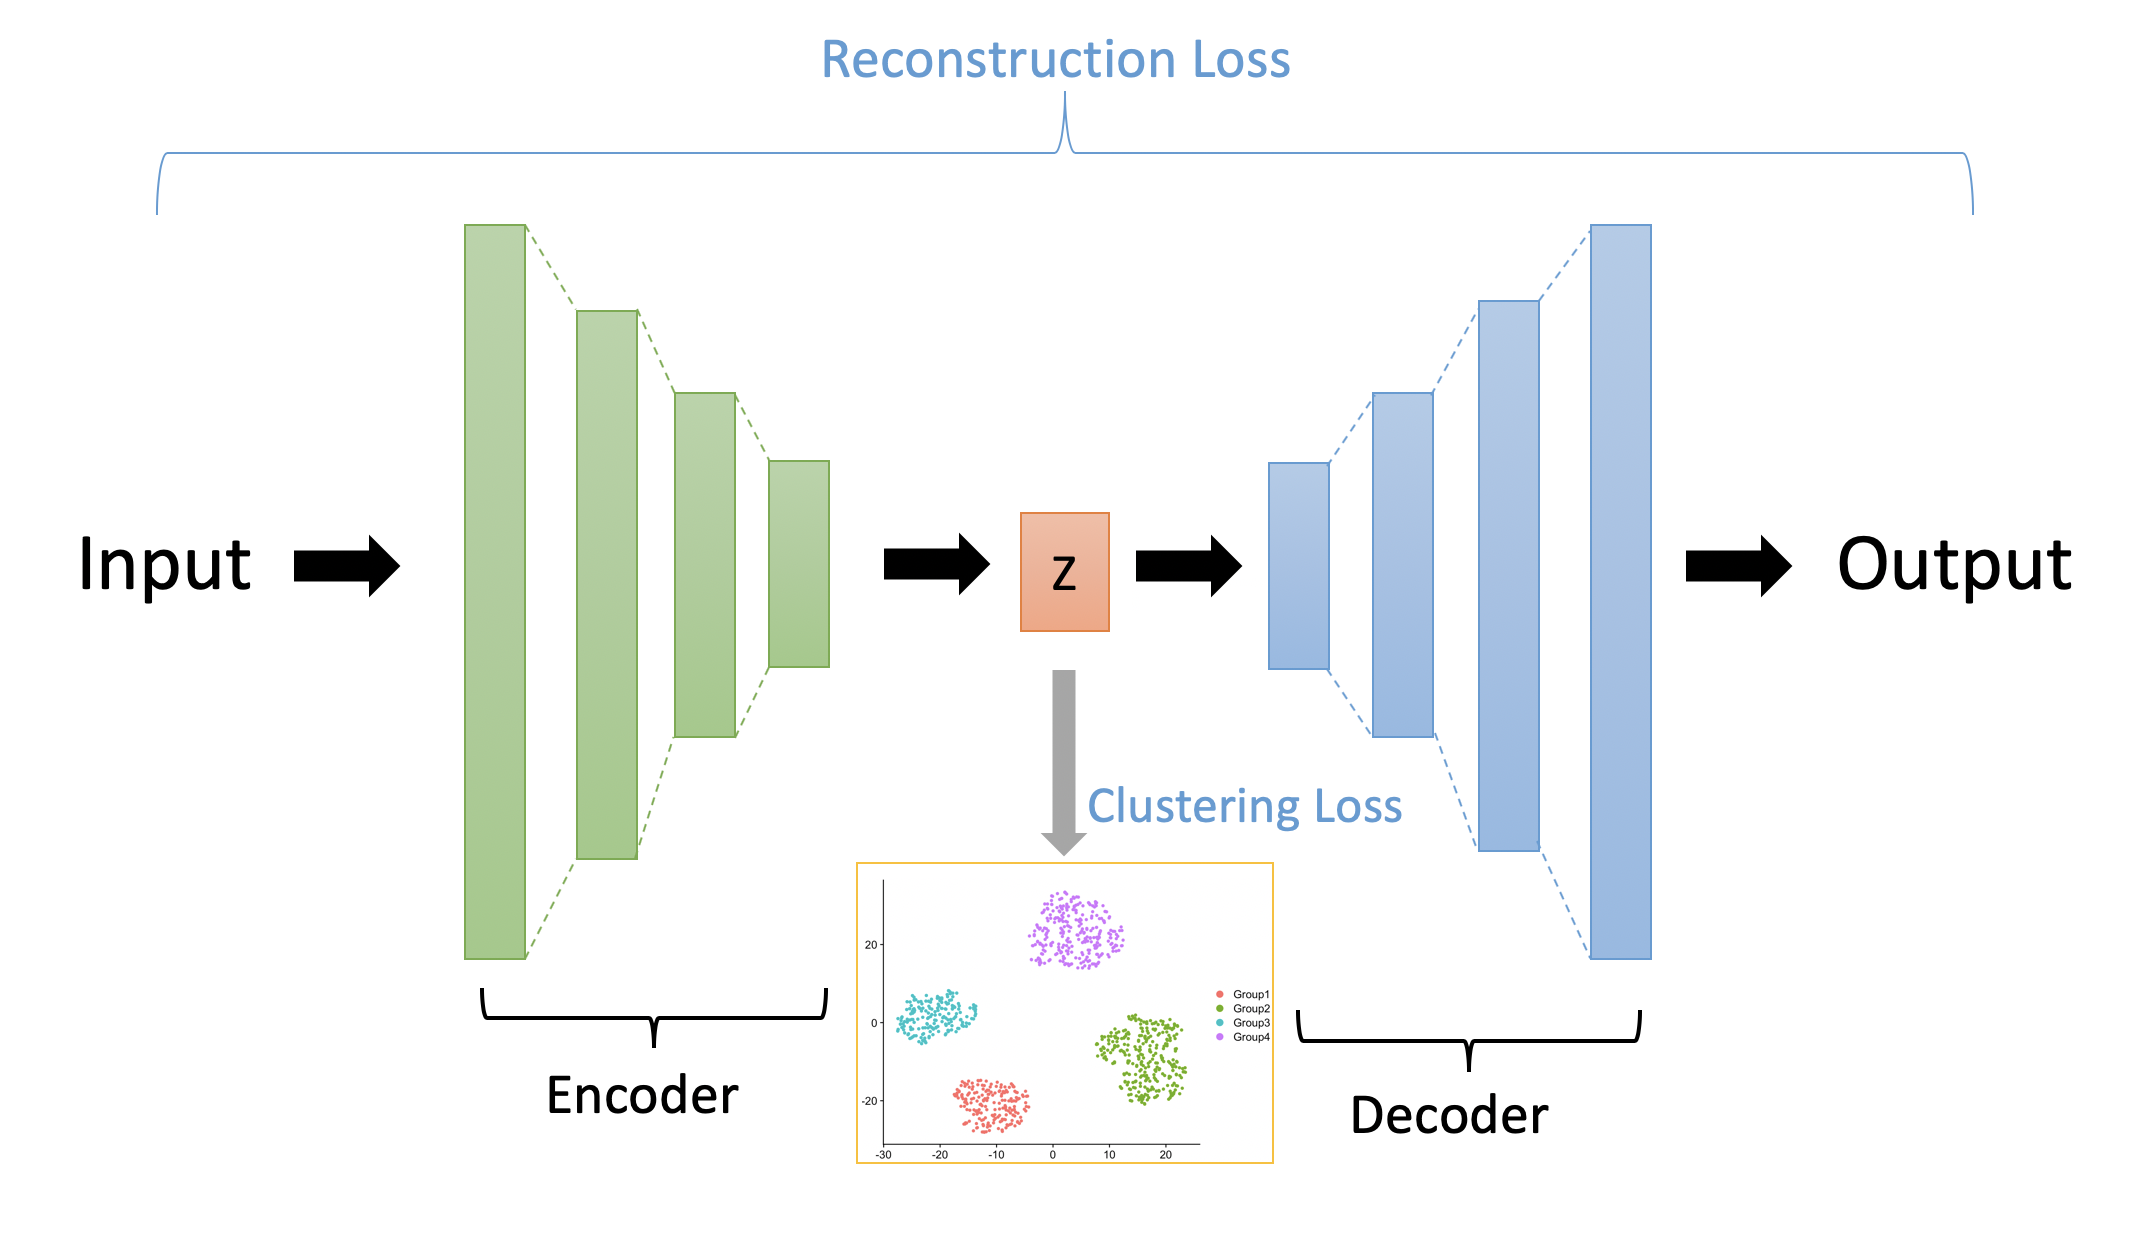
\includegraphics[width=1\textwidth]{figures/myfigures/dc.png}
    \caption{The structure of the deep clustering model}
    \label{dcstru}
\end{figure}

For the clustering process, we tried four methods: the spectral clustering \cite{von2007tutorial}, DBSCAN \cite{ester1996density}, K-means \cite{kanungo2002efficient} and Louvain methods \cite{traag2019louvain}. The Louvain method can achieve better visualization performance than the other three methods. However, the overall result is not good enough now. We are still trying to optimize the model.

It is also worth trying to reduce the dimensionality and infer the cell lineage jointly. Unlike performing clustering tasks in latent space in deep clustering methods, we can constrain the latent variables to form a tree structure or a graph structure, thus getting the latent variables that are friendly for trajectory inference.

The optimization of this kind of model consists of two parts. Firstly, pre-train the network as a normal variational autoencoder. Then, performing alternating training to optimize clustering loss and reconstruction loss at the same time.

\subsubsection{GAN for scRNA-seq data}
Generative Adversarial Networks \cite{radford2015unsupervised} are extensively used for unsupervised representation learning in recent years. In a single-cell data analysis domain, it has been used for dimensionality reduction \cite{lin2020deep}, data generation, and data augmentation \cite{marouf2018realistic}. For dimensionality reduction, the structure in the figure can be used. In this model, the loss function in the variational autoencoder is replaced by a discriminator, a multi-layer neuron network with decreasing unit layers. Because of the dropout events, using pair-wise distance to measure the difference between two expression matrix can be inaccurate. In this way, the discriminator can learn more complex functions to distinguish the true expression and generated expression than the simple mean squared error function. Moreover, the discriminator network can also be combined with other models, such as the clustering-friendly dimensionality reduction model and the ZIVA model, to generate more powerful methods. 

\begin{figure}[htb!]
    \centering
    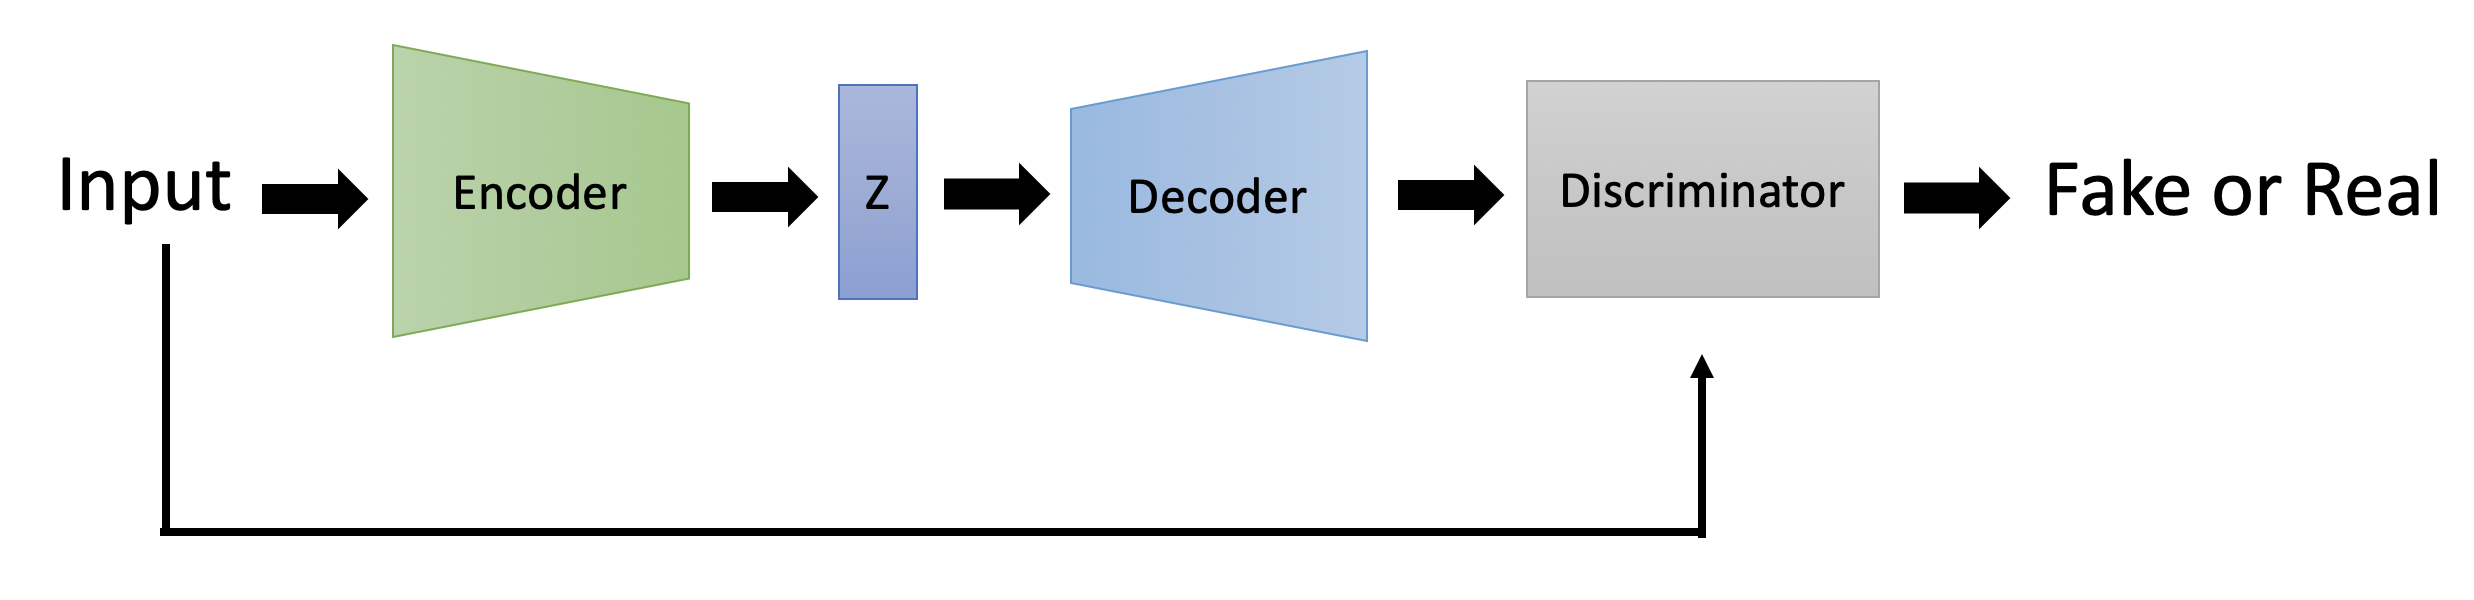
\includegraphics[width=1\textwidth]{figures/myfigures/vaegan.png}
    \caption{The structure of the VAE-GAN model}
    \label{dcstru}
\end{figure}

\subsubsection{GVAE for scRNA-seq data}
In recent years, graph neuron network has been widely used in various industries such as social network \cite{yang2016revisiting}, recommendation systems \cite{kipf2016semi}. Single-cell sequencing data can also be viewed as a graph where each node is a cell. For example, a study \cite{ravindra2020disease} uses graph convolutional neuron network \cite{velivckovic2017graph} to predict the disease state of Multiple Sclerosis. The graph structure can also be applied to the variational autoencoder model \cite{kipf2016variational}. It is possible that through the preservation of the graph structure of single cells in high dimensionality spaces, variational graph autoencoder can have better dimensionality reduction performance on global cell structures.

   